%%
%% This is file `tikzposter-example.tex',
%% generated with the docstrip utility.
%%
%% The original source files were:
%%
%% tikzposter.dtx  (with options: `tikzposter-example.tex')
%% 
%% This is a generated file.
%% 
%% Copyright (C) 2014 by Pascal Richter, Elena Botoeva, Richard Barnard, and Dirk Surmann
%% 
%% This file may be distributed and/or modified under the
%% conditions of the LaTeX Project Public License, either
%% version 2.0 of this license or (at your option) any later
%% version. The latest version of this license is in:
%% 
%% http://www.latex-project.org/lppl.txt
%% 
%% and version 2.0 or later is part of all distributions of
%% LaTeX version 2013/12/01 or later.
%% 








% Default values for poster format options.
\documentclass[25pt, a0paper, portrait, margin=0mm, innermargin=15mm,
    blockverticalspace=15mm, colspace=15mm, subcolspace=8mm]{tikzposter}

% \tikzposterlatexaffectionproofon %shows small comment on how the poster was made at bottom of poster
\tikzposterlatexaffectionproofoff %don't show small comment on how the poster was made at bottom of poster

% Commands
\newcommand{\bs}{\textbackslash}   % backslash
\newcommand{\cmd}[1]{{\bf \color{red}#1}}   % highlights command

% Title, Author, Institute
\title{Estimating pseudotime: ordering single-cell data}
\author{John Reid, Lorenz Wernisch}
\institute{MRC Biostatistics Unit, Cambridge, UK}

% -- PREDEFINED THEMES ---------------------- %
% Choose LAYOUT:  Default, Basic, Rays, Simple, Envelope, Wave, Board, Autumn, Desert,
\usetheme{Simple}
\usecolorstyle[colorPalette=Default]{Default}

\usepackage{graphicx}
\usepackage{layouts}


\begin{document}

\maketitle

\begin{columns}%blocks will be placed into columns
\column{.5}
\block[roundedcorners=40]{Introduction}{
    
    Our understanding of dynamical biological systems such as developmental
    processes or transitions into disease states is limited by our ability to
    reverse-engineer these systems using data available from high-throughput
    experimental protocols. Protocols such as single cell RNA-seq are
    destructive in nature, generating cross-sectional time series in which it
    is not possible to track the progress of one sample through the system. In
    contrast, longitudinal data would be far more suitable for
    reverse-engineering these systems but currently there are no
    high-throughput protocols that can generate it.
}

\block[roundedcorners=40]{Pseudotime}{
    Individual cells progress through these systems at different rates, thus a sample's
    experimental capture time may not accurately reflect how far it has progressed. We
    propose a probabilistic model that relies on some smoothness assumptions to estimate and
    correct for this effect. Each cell is assigned a pseudotime that represents its progress
    through the system. These pseudotimes are related to but not determined by the cells'
    experimental capture times.

    % Text width is \printinunitsof{in}\prntlen{\textwidth}.

    \begin{tikzfigure}[
        Simulated data to illustrate the relationship between
        capture times (top) and pseudotimes (bottom). Our model uses a
        smoothness assumption across the expression profiles of several genes
        to estimate pseudotimes. Conversely our method can be seen as
        estimating a noise decomposition into intrinsic measurement
        noise and noise introduced by grouping cells that have progressed
        at different rates by capture time.]
        \label{fig:capture-pseudo}
        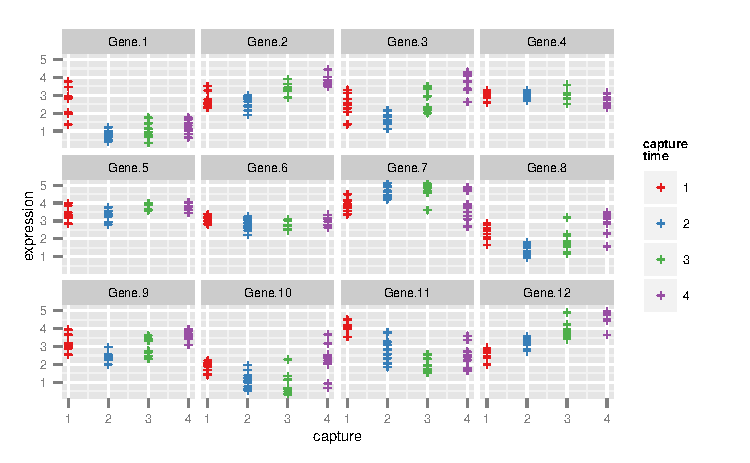
\includegraphics[width=.99\linewidth]{Figures/capture-multi}
        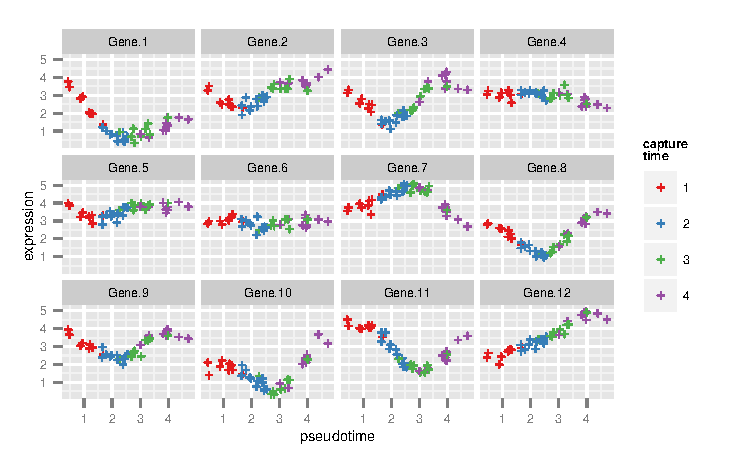
\includegraphics[width=.99\linewidth]{Figures/pseudo-multi}
    \end{tikzfigure}
}

\block{Model}{
    We model the smoothness assumption on each gene's expression profile $y_g$
    using a Gaussian process over pseudotime. Gene-specific parameters in the
    covariance function represent intrinsic measurement noise $\omega_g$
    and variation of the profile over time $\psi_g$. Each sample's
    pseudotime $\tau_c$ is given a normal prior centred on its capture time.
    \begin{eqnarray}
      y_{g} &\sim& \mathcal{GP}(\phi_g, \Sigma_g) \nonumber\\
      \Sigma_g(\tau_1, \tau_2)
        &=& \psi_g \Sigma_\tau(\tau_1, \tau_2)
            + \omega_g \delta_{\tau_1,\tau_2} \nonumber\\
      \log \psi_g &\sim& \mathcal{N}(\mu_\psi, \sigma_\psi) \nonumber\\
      \log \omega_g &\sim& \mathcal{N}(\mu_\omega, \sigma_\omega) \nonumber\\
        \Sigma_\tau(\tau_1, \tau_2)
            &=& \textrm{Matern}_{3/2}\bigg(r=\frac{|\tau_1 - \tau_2|}{l}\bigg)
            = (1 + \sqrt{3}r) \exp[-\sqrt{3}r] \nonumber\\
      \tau_c &\sim& \mathcal{N}(k_c, \sigma_\tau) \nonumber
    \end{eqnarray}
    This model is effectively a one-dimensional Gaussian process latent
    variable model with a structured prior on the latent variable (pseudotime).
}

\column{.5}
\block{\emph{Arabidopsis} response to infection}{

    To test our model's performance we validated it by obfuscating capture
    times from a high-resolution data set generated by Windram et al.
    (The Plant Cell 2012) that studies the response of \emph{Arabidopsis}
    to infection.  The original data had 24 distinct
    capture times, we grouped these into four groups and asked the model
    to infer pseudotimes. In order to quantify the smoothness of our
    pseudotime assignments, we defined a roughness statistic:
    \[
    R_g(z) = \frac{1}{\sigma_g}
        \sqrt{\frac{1}{C-1}\sum_{c=1}^{C-1} (x_{g,z_c}-x_{g,z_{c+1}})^2}
    \]
    \begin{tikzfigure}[\emph{Left}: Expression profiles over pseudotime
        coloured by group.
        \emph{Right}: Roughness statistics (red) from the posterior of our
        model compared to a random pseudotime orderings (green). The
        roughness statistic of the sample with the best likelihood is shown
        as a dotted line.]
        \label{fig:Windram}
        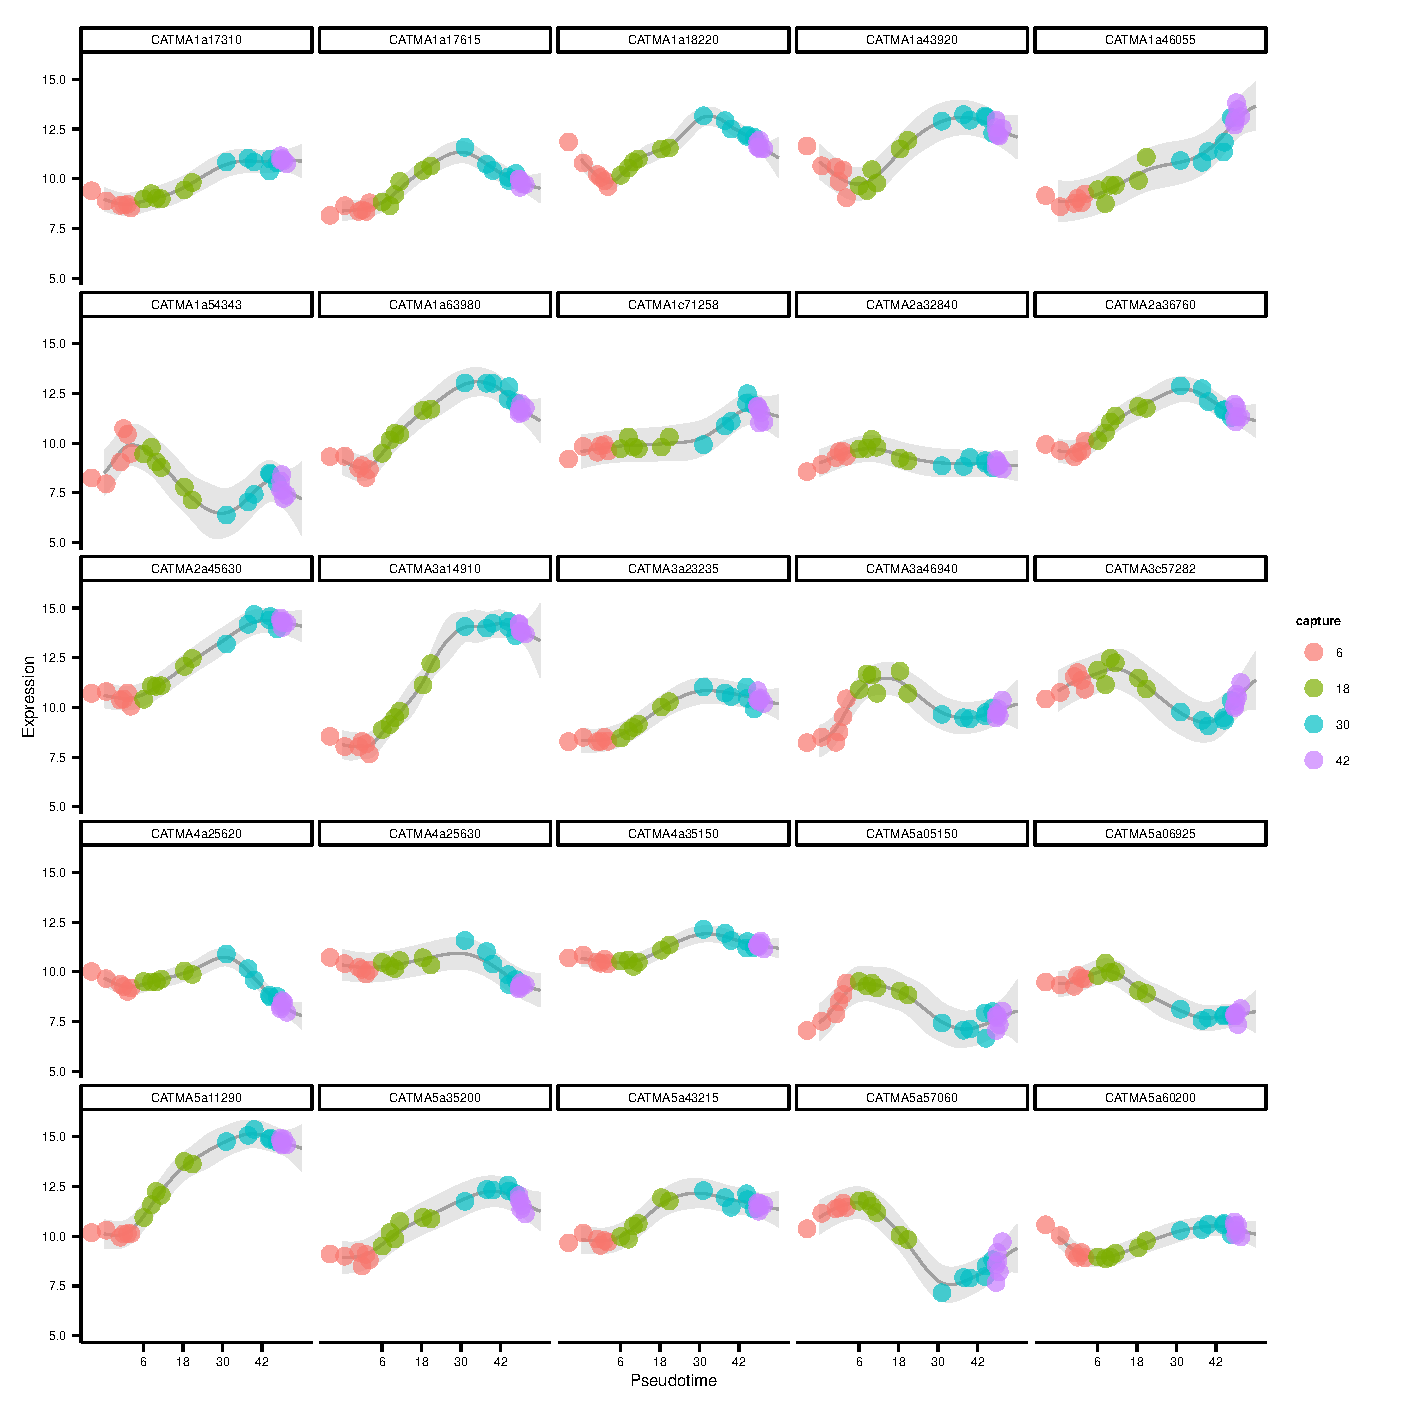
\includegraphics[width=.99\linewidth]{Figures/Windram-profiles}
        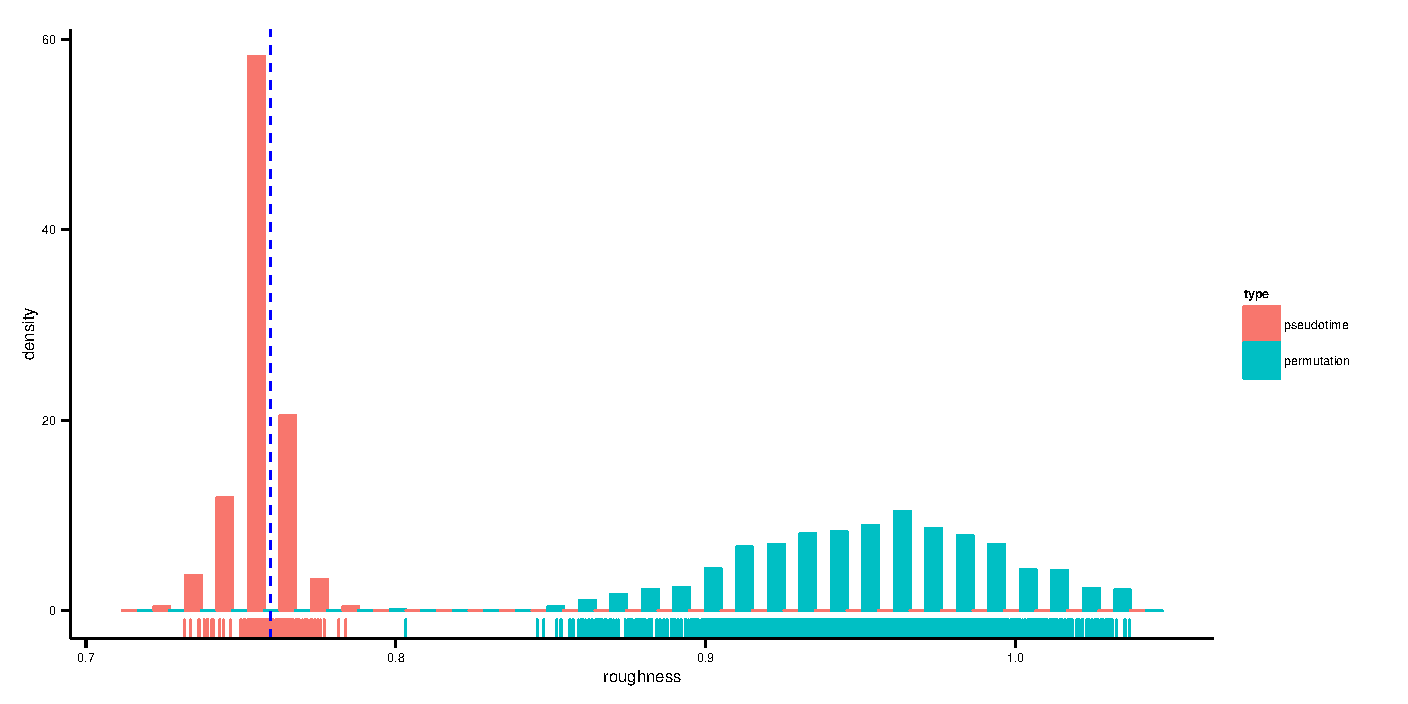
\includegraphics[width=.99\linewidth]{Figures/Windram-roughnesses}
    \end{tikzfigure}
}

\block{Paracrine signalling in mouse dendritic cells}{
    Shalek et al. (Nature 2014) used single cell RNA-seq to study paracrine
    signalling
    in mouse dendritic cells. They identified two precocious cells captured
    at the 1 hour time point that had progressed further through the system.
    Our model successfully identified these cells,
    placing them in the midst of cells captured at two hours.

    \begin{tikzfigure}[\emph{Left}: Expression profiles over pseudotime
        \emph{Right}: Roughness statistics as above.]
        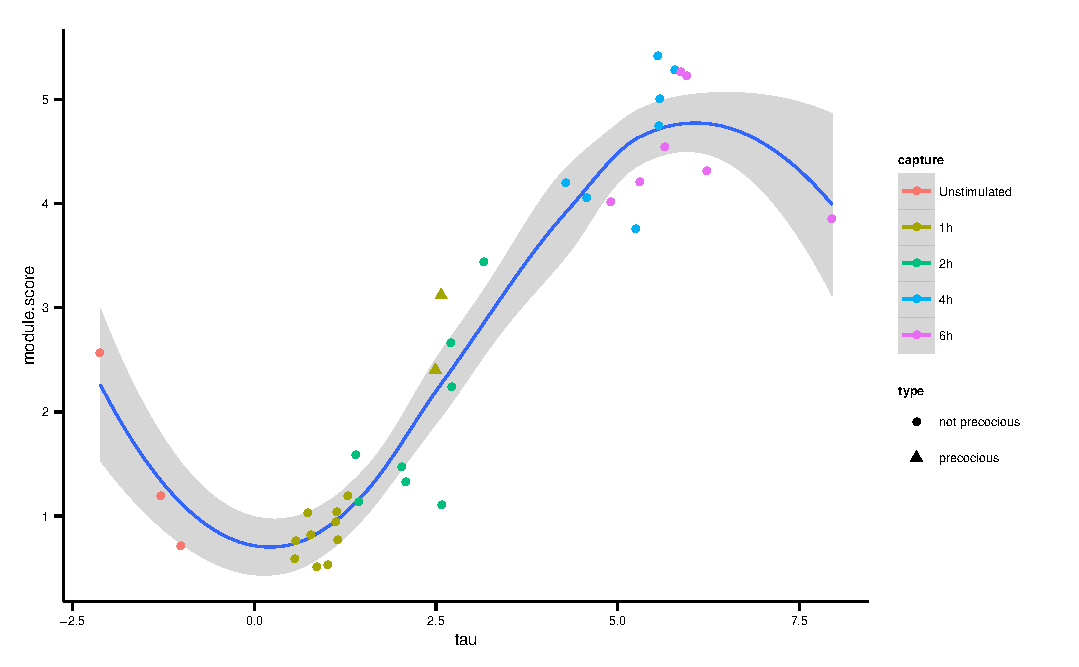
\includegraphics[width=.49\linewidth]{Figures/Shalek-core}
        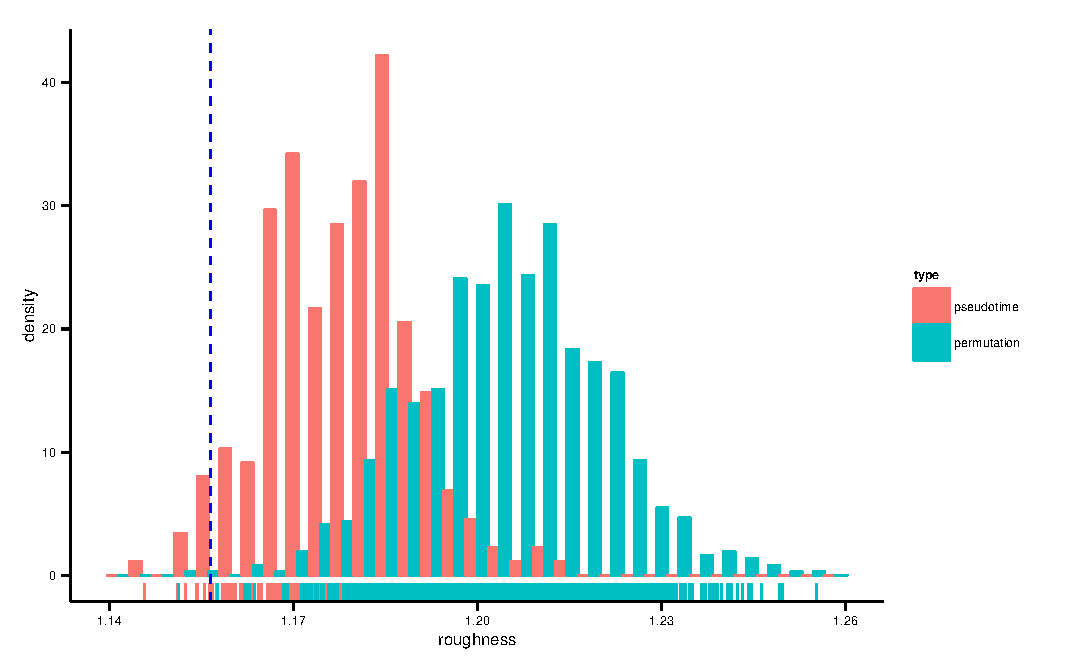
\includegraphics[width=.49\linewidth]{Figures/Shalek-roughnesses}
        \label{fig:Shalek}
    \end{tikzfigure}
}

\end{columns}

\end{document}

\endinput
%%
%% End of file `tikzposter-example.tex'.
